% !TeX program = lualatex -shell-escape
%
% The above is a magic comment recognized by Textmate, TeXShop, TeXstudio, and TeXworks 
% =======================================================================
%  AI-Assisted Shortcuts Plugin for PyMOL 3.0
%  32-slide Beamer talk with figure placeholders and speaker notes
%
%  Speaker notes:
%    - Notes appear via \note{...} on each frame.
%    - To display them, uncomment ONE of the two lines just below
%      \begin{document}. "show notes on second screen=right" is handy
%      when presenting with a projector plus a laptop screen.
%
%  Figure placeholders:
%    - \figph{...} draws a gray box with a caption of what belongs there.
%    - Replace each \figph{...} with \includegraphics{...} when the real
%      figure is ready.
%=======================================================================

%  <<<<<  uncomment to generate handouts   >>>>>>
% %  <<<<<  comment to generate slides   >>>>>>
% \documentclass[handout,letter]{beamer}
% \RequirePackage{luatex85}
%
% \usepackage{pgfpages}
% \mode<handout>{\pgfpagesuselayout{2 on 1}[letterpaper, border shrink = 1mm]}
% \setbeameroption{show notes}
% \setbeamercolor{note page}{bg=white}
% \setbeamertemplate{note page}{\insertnote\par}
% \setbeamerfont{note page}{size=\footnotesize}
% %\addtobeamertemplate{note page}{\setbeamerfont{itemize/enumerate subbody}{size=\footnotesize}}{}
% \setbeamersize{text margin left=0em,text margin right=0em}
% \addtobeamertemplate{note page}{\setlength{\parskip}{4pt}}
% % >>>>>>
%

%%%%%% <<<<<  comment above and uncomment below to generate slides only   >>>>>>
\documentclass[aspectratio=169,11pt]{beamer}
%%% >>>>>>


% \newminted{python}{fontsize=\normalsize,
%                    linenos=false,
%                    numbersep=8pt,
%                    gobble=4,
%                    breaklines,
%                    frame=lines,
%                    bgcolor=bgpython,
%                    framesep=3mm}
%
% \newminted{bash}{fontsize=\largesize,
%                    linenos=false,
%                    numbersep=8pt,
%                    breaklines,
%                    gobble=4,
%                    frame=lines,
%                    bgcolor=bgbash,
%                    framesep=3mm}
%
% \definecolor{bgpython}{rgb}{0.95,0.95,0.95}
% \definecolor{bgbash}{rgb}{0.95,0.85,0.75}

% \setsansfont{TeX Gyre Heros}
% \setbeamerfont{note page}{family*=pplx,size=\footnotesize} % Palatino for notes
% "TeX Gyre Heros can be used as a replacement for Helvetica"
% In Unix, unzip the following into ~/.fonts
% In Mac, unzip it, double-click the .otf files, and install using "FontBook"
%   http://www.gust.org.pl/projects/e-foundry/tex-gyre/heros/qhv2.004otf.zip

\RequirePackage{luatex85}
\usepackage{animate}
\usepackage{pgfpages}
\usepackage{moresize}
\usetheme{default}
\beamertemplatenavigationsymbolsempty
\hypersetup{pdfpagemode=UseNone} % don't show bookmarks on initial view
%tables
\usepackage{booktabs}% http://ctan.org/pkg/booktabs
% font
\usepackage{amsmath}
\usepackage{amssymb}
\usepackage{minted}
\usepackage{fix-cm}
\usepackage{fontspec}
\usepackage{gensymb}
\usepackage{tabularx,booktabs}
\usepackage{enumitem}

%\usetheme{Madrid}
%\usecolortheme{seahorse}
%\useinnertheme{rectangles}
%\setbeamertemplate{navigation symbols}{}   % remove navigation clutter
\setbeamertemplate{caption}[numbered]

% Approximate Arial with a clean sans-serif face
\usepackage[T1]{fontenc}
\usepackage{helvet}
\renewcommand{\familydefault}{\sfdefault}

\usepackage{graphicx}
%\usepackage{booktabs}
\usepackage{xcolor}
\usepackage{tikz}

% Center the title and increase its size
\setbeamertemplate{frametitle}[default][center]
\setbeamerfont{frametitle}{size=\huge}


% named colors
\definecolor{offwhite}{RGB}{249,242,255}
\definecolor{foreground}{RGB}{25,25,25}
\definecolor{background}{RGB}{255,255,255}
\definecolor{title}{RGB}{100,0,0}
\definecolor{gray}{RGB}{155,155,155}
\definecolor{subtitle}{RGB}{50,0,0}
\definecolor{hilight}{RGB}{102,255,204}
\definecolor{vhilight}{RGB}{255,111,207}
\definecolor{lolight}{RGB}{155,155,155}
%\definecolor{green}{RGB}{125,250,125}

% use those colors
\setbeamercolor{titlelike}{fg=title}
\setbeamercolor{subtitle}{fg=subtitle}
\setbeamercolor{institute}{fg=gray}
\setbeamercolor{normal text}{fg=foreground,bg=background}
\setbeamercolor{item}{fg=foreground} % color of bullets
\setbeamercolor{subitem}{fg=gray}
\setbeamercolor{itemize/enumerate subbody}{fg=gray}
\setbeamertemplate{itemize subitem}{{\textendash}}
\setbeamerfont{itemize/enumerate subbody}{size=\footnotesize}
\setbeamerfont{itemize/enumerate subitem}{size=\footnotesize}
\setbeamercolor{section in toc}{fg=title}
\setbeamercolor{caption name}{fg=title}

% page number
\setbeamertemplate{footline}{%
    \raisebox{5pt}{\makebox[\paperwidth]{\hfill\makebox[20pt]{\color{gray}
          \scriptsize\insertframenumber}}}\hspace*{5pt}}

% add a bit of space at the top of the notes page
\addtobeamertemplate{note page}{\setlength{\parskip}{12pt}}

% a few macros
\newcommand{\bi}{\begin{itemize}[font=$\bullet$\scshape\bfseries]}
\newcommand{\ei}{\end{itemize}}
\newcommand{\ig}{\includegraphics}
\newcommand{\subt}[1]{{\footnotesize \color{subtitle} {#1}}}

\usepackage{latexsym} % for squares for the check-list environment
\newenvironment{checklist}{%
  \begin{list}{}{}% whatever you want the list to be
  \let\olditem\item
  \renewcommand\item{\olditem[$\Box$] }
}{%
  \end{list}
}




% ---- Figure placeholder command -------------------------------------
% Usage: \figph[width]{description text}
\newcommand{\figph}[2][0.72\linewidth]{%
  \setlength{\fboxsep}{0pt}%
  \begin{center}%
  \fcolorbox{gray!60}{gray!12}{%
    \parbox[c][3.4cm][c]{#1}{\centering\itshape\small
      [Figure placeholder]\\[2pt]#2}}%
  \end{center}%
}

% ---- Metadata -------------------------------------------------------
\title[]{Teaching Crystallographic Computing with Computational Notebooks}
\author{\textbf{Blaine Mooers, PhD} \\ blaine-mooers@ou.edu }
\institute[OUHC]{Department of Biochemistry and Physiology, University of Oklahoma Health Campus,\\ Oklahoma City, Oklahoma}
\date{2026 August 17 \\ Teaching Computational Crystallography Minisymposium\\ 27th Congress and General Assembly of the IUCr\\ Calgary, Alberta \\ \url{github.com/MooersLab/iucr2026-teaching-computational-crystallography}}

\subsection{Title slide}

\title{Teaching Crystallographic Computing with Computational Notebooks}
\author{\textbf{Blaine Mooers, PhD \\ blaine-mooers@ou.edu}}
\institute{{Department of Biochemistry \& Physiology}\\[2pt]{University of Oklahoma Health Sciences Center, Oklahoma City} }
\date{IUCr 2026 \\ 2016 August 17, 3:00-3:30 PM, Room 224 \\  \vfill  Slides and notebooks: \\ \url{MooersLab/iucr2026-teaching-computational-crystallography}}


% =======================================================================
\begin{document}

% To show speaker notes, uncomment exactly one of the following:
%\setbeameroption{show notes}
%\setbeameroption{show notes on second screen=right}

%--------------------------------------------------- Slide 1: Title
\begin{frame}[plain]
  \titlepage
\end{frame}
\note{
Welcome to this presentation on teaching crystallographic computing with computational notebooks.
I will share strategies developed over a decade of teaching structural biology methods to first-year graduate students in the biomedical sciences.
The core idea is to embed computational notebook demonstrations into existing lectures rather than creating standalone courses.
This approach addresses the practical reality that dedicated courses in computational crystallography are rare and curriculum space is limited.

This presentation aligns with the longstanding mission of the IUCr Commission on Crystallographic Computing (CompComm), established in 1959 to promote the collection and dissemination of information relating to crystallographic computing.
The Commission has consistently emphasized the need to train new generations of crystallographers capable of understanding and extending computational tools.
}

\begin{frame}{Outline}
  \tableofcontents[hideallsubsections]
\end{frame}
\note{I will cover my motivation, the features of the plugin, why the shortcuts still matter in the age of AI, and how AI can work with the shortcuts..}


%%%%%%%%%%%%%%%%%%%%  2  %%%%%%%%%%%%%%%%%%%%%%%%%%%%%%%%%%%%%%%%%%%%
\section{The Curriculum Challenge and One Approach}
\subsection{Limited Opportunities}
\begin{frame}[fragile]
\frametitle{The Curriculum Challenge}
\Large{
\begin{itemize}[font=$\bullet$\scshape\bfseries]
    \item Limited opportunities for teaching crystallography.
    \item Even more limited opportunities for teaching computational crystallography.
    \item Intense competition for slots in first year graduate curricula.  
    \item Graduate students arrive with limited computing experience.
    \item Limited to covering these topics in group meetings and day long workshops.  
\end{itemize}
}
\end{frame}
\note{
The curriculum landscape for crystallography has become increasingly challenging.
Most PIs will never have the opportunity to teach a formal course in crystallography, let alone one focused on computational methods.
Department curriculum committees often favor newer techniques like cryo-EM data analysis when allocating limited teaching slots.
This creates a gap in training that affects the next generation of structural biologists.

The IUCr Computing Commission recognized this challenge years ago.
A joint Computing Commission/Teaching Commission newsletter on ``Age Concern'' (2009) addressed ``the slow march towards retirement of the major generation of crystallographic programmers.''
The newsletter warned that ``few young crystallographers are nowadays capable to read the source code of widely used programs'' and expressed concern about software becoming ``binary format only and thus not extendable.''
This concern about training continuity remains urgent today.
}


%%%%%%%%%%%%  3  %%%%%%%%%%%%%%%%%%%%%%%%%%%%%%%%%%%%%%%%%%%%
\subsection{The Stealthy Solution}
\begin{frame}[fragile]
\frametitle{Solution: embed vignettes in existing lectures}
\Large{
\begin{itemize}[font=$\bullet$\scshape\bfseries]
    \item Limit to a short vignette of several notebook cells; do not have to run full notebook.
    \item No need for new course approvals.
    \item Minimal disruption to existing curricula.
    \item Reduces the abstract nature of crystallographic concepts.
\end{itemize}
}
\end{frame}
\note{
My response to these constraints is to take a stealthy approach.
Rather than proposing new courses that require committee approval and curriculum reorganization, I incorporate computational notebook demonstrations directly into existing lectures.
This approach leverages software development skills over formal pedagogical training.
The key insight is that seeing code executed in real-time makes abstract crystallographic concepts concrete and appear more accessible.

This philosophy aligns with the 2023 Melbourne Crystallographic Computing School, which welcomed ``all ages and all levels of experience'' with only ``a basic knowledge in crystallography and a basic knowledge of programming'' required.
A February 2025 paper in \textit{Journal of Applied Crystallography} on crystallographic education advocates hands-on approaches that ``ensure students gain a lasting memory of what they learned'' and can ``ignite their excitement about the capabilities of structural science.''
}




%%%%%%%%%%%%%%%%%%%%  4  %%%%%%%%%%%%%%%%%%%%%%%%%%%%%%%%%%%%%%%%%%%%
\section{The Computational Notebook Platform}
\subsection{What Are Computational Notebooks?}
\begin{frame}[fragile]
\frametitle{What Are Computational Notebooks?}
\begin{columns}
     \begin{column}{0.70\linewidth}
\begin{itemize}[font=$\bullet$\scshape\bfseries]
    \item Computational narratives that combind executable code, output, and text.
    \item Jupyter notebooks are the most widely used format.
    \item Jupyter: Julia, Python, and R.
    \item Support polyglot computing via kernels.
    \item Students see cause and effect.
    \item Dopamine hits from instant gratification.
    \item Uses: code chunk developement, data exploration, teaching, self-directed tutorials, and supplemental materials.
\end{itemize}
\end{column}
\begin{column}{0.28\linewidth}
      \begin{figure}
        \centering
        
\includegraphics[width=\linewidth]{./figs/logos-jupyter}
      \end{figure}
   \end{column}
 \end{columns}
 \vfill
\footnotesize{Kluyver et al. (2016)  In F. Loizides \& B. Schmidt (Eds.), Positioning and Power in Academic Publishing: Players, Agents and Agendas (pp. 87–90). IOS Press. }
\end{frame}
\note{
Computational notebooks, particularly Jupyter notebooks, have become a standard tool in data science and scientific computing.
They combine executable code with explanatory text and visualizations in a single document.
For teaching, they offer the crucial advantage that students can see how code produces results in real-time.
This immediate feedback helps build intuition about crystallographic algorithms.

A 2023 paper in \textit{Journal of Applied Crystallography} on ``FAIR and scalable management of small-angle X-ray scattering data'' explicitly used ``the programming language Python, the widely used computing platform Jupyter Notebook'' to achieve FAIR compliance.
This establishes precedent within the crystallographic community for notebooks as vehicles for reproducible research.
The 2020/2021 Nov\'{e} Hrady Computing School, held online due to the pandemic, demonstrated the Commission's adaptability to remote education---a format that computational notebooks are ideally suited to support.
}

%%%%%%%%%%%%%%%%%%%%  5  %%%%%%%%%%%%%%%%%%%%%%%%%%%%%%%%%%%%%%%%%%%%

\begin{frame}[fragile]
\frametitle{Platforms for Jupyter}
\Large{
\begin{itemize}[font=$\bullet$\scshape\bfseries]
    \item \textbf{Jupyter Lab}:  (+) recommended, (+) IDE-like.
    \item Jupyter Notebook: (+) Classic and (+) modern variants.
    \item nteract.app: (+) drag-and-drop install, (-) no extensions.
    \item Google Colab: (+) no local install problems, (-) time-consuming virtual machine setup.
\end{itemize}
}
\end{frame}
\note{
}


\begin{frame}[fragile]
\frametitle{Six demonstration notebooks}
The notebooks are coded to run in Google Colab and Jupyter. Corresponding Python scripts are included.
\begin{itemize}[font=$\bullet$\scshape\bfseries]
    \item Demo 1: Data reduction with DIALS and Gemmi. Downloads images from Zenodo
    \item \textbf{Demo 2: Data reduction with XDS.}
    \item \textbf{Demo 3: MR with Phaser}
    \item \textbf{Demo 4: Refinement with Phenix}
    \item Demo 5: Advanced data analysis with reciprocalspaceship
    \item Demo 6: Code reuse.
\end{itemize}
\vfill
\emph{If the software has a Python API or binaries that can be run in the terminal, you can run them in Jupyter.}
\end{frame}
\note{
}


%%%%%%%%%%%%%%%%%%%%  7  %%%%%%%%%%%%%%%%%%%%%%%%%%%%%%%%%%%%%%%%%%%%
\section{Six Notebooks}
\subsection{DIALS in Jupyter}
\begin{frame}[fragile]
\frametitle{DIALS in Jupyter}
DIALS:  Diffraction Integration for Advanced Light Sources
\begin{center}
% \Large{\textbf{LIVE DEMONSTRATION}}
% \vspace{1em}

\begin{columns}
\begin{column}{0.68\linewidth}
\textbf{Topics covered:}
\begin{itemize}[font=$\bullet$\scshape\bfseries]
    \item Importing diffraction images from Zenodo
    \item Spot finding and indexing
    \item Refinement and integration
    \item Visualizing reciprocal space
\end{itemize}
\end{column}

\begin{column}{0.28\linewidth}
\begin{figure}
    \centering
    
\includegraphics[width=\linewidth]{./figs/logo-DIALS}
    \end{figure}
\end{column}
\end{columns}
\end{center}
\footnotesize{DIALS: Winter et al. (2018) Acta Cryst. Sect. D 74, 86-97; 6YNQ: Gunther  et al.  (2021) Science 372, 642-646.}
\end{frame}
\note{
Now I will switch to a live Jupyter notebook to demonstrate DIALS.
This notebook shows how to import diffraction images, perform spot finding, and carry out indexing.
Students can modify parameters and immediately see how results change.
The notebook includes inline visualizations of reciprocal space that help students understand the geometry of diffraction data.

DIALS was designed as ``a framework rather than a monolithic integration program'' that ``facilitates the construction of various alternative workflows for performing data-reduction tasks.''
This extensible architecture makes it particularly well-suited for educational demonstrations where we want to expose the underlying algorithms.
}


%%%%%%%%%%%%%%%%%%%%  8  %%%%%%%%%%%%%%%%%%%%%%%%%%%%%%%%%%%%%%%%%%%%
\subsection{XDS via Subprocess Calls}
\begin{frame}[fragile]
\frametitle{XDS via Subprocess Calls}
XDS: X-ray Detector Software
\begin{center}
% \Large{\textbf{DEMONSTRATION}}
% \vspace{1em}
\begin{columns}
    \begin{column}{0.68\linewidth}
\textbf{Topics covered:}
\begin{itemize}[font=$\bullet$\scshape\bfseries]
    \item Generate XDS.INP file.
    \item Run XDS from notebook cells.
    \item Parse CORRECT.LP for statistics.
    \item Compare results with DIALS.
\end{itemize}
\end{column}
\begin{column}{0.28\linewidth}
\begin{figure}
    \centering
    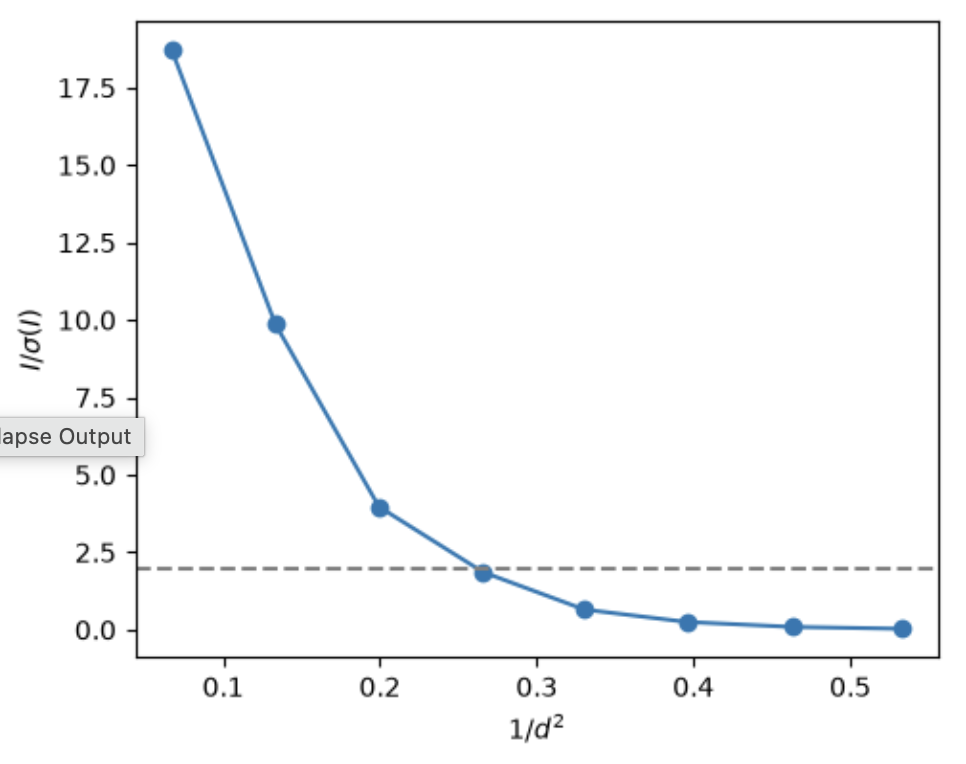
\includegraphics[width=\linewidth]{./figs/xds}
    \end{figure}
\end{column}
\end{columns}
\end{center}
\footnotesize{Kabsch (2010) Acta Cryst. Sect. D 66, 125-132.}
\end{frame}
\note{
XDS uses a different interface model based on input files.
This notebook demonstrates how to generate XDS.INP files programmatically and run XDS through subprocess calls.
I parse the output files to extract key statistics and display them in the notebook.
Comparing XDS and DIALS results on the same dataset helps students understand that different software can produce similar results through different algorithmic approaches.

This comparison exemplifies the Commission's encouragement of ``diversity in crystallographic software development.''
Students learn that multiple valid approaches exist and develop critical evaluation skills rather than becoming dependent on a single tool.
}


%%%%%%%%%%%%%%%%%%%%  10  %%%%%%%%%%%%%%%%%%%%%%%%%%%%%%%%%%%%%%%%%%%%
\subsection{Molecular Replacement Demo}
\begin{frame}[fragile]
\frametitle{Molecular Replacement Workflow}
\begin{center}
% \Large{\textbf{LIVE DEMONSTRATION}}
% \vspace{1em}
\begin{columns}
    \begin{column}{0.68\linewidth}
\textbf{Topics covered:}
\begin{itemize}[font=$\bullet$\scshape\bfseries]
    \item Preparing search models with CHAINSAW or Gemmi.
    \item Running PHASER.
    \item Evaluating MR solutions.
    \item Initial refinement cycles.
\end{itemize}
\end{column}
\begin{column}{0.28\linewidth}
\begin{figure}
    \centering
    
\includegraphics[width=\linewidth]{./figs/logo-phaser}
    \end{figure}
\end{column}
\end{columns}
\end{center}
\footnotesize{McCoy, A. J. et al. (2007). J. Appl. Cryst. 40, 658-674.}
\end{frame}
\note{
This demonstration walks through a complete molecular replacement workflow.
I start with model preparation using CHAINSAW to trim a homologous structure.
Then I run the molecular replacement search and show students how to evaluate whether the solution is correct.
The notebook captures the entire workflow in a reproducible format that students can adapt for their own projects.

This integration across the pipeline---from model preparation through initial refinement---extends beyond what Commission schools have typically covered in isolation.
By showing the complete workflow, students gain appreciation for how individual steps connect into a coherent structure determination process.
}


%%%%%%%%%%%%%%%%%%%%  12  %%%%%%%%%%%%%%%%%%%%%%%%%%%%%%%%%%%%%%%%%%%%
\subsection{Refinement Workflow}
\begin{frame}[fragile]
\frametitle{Refinement Workflow}
\begin{center}
% \Large{\textbf{LIVE DEMONSTRATION}}
% \vspace{1em}
\begin{columns}
\begin{column}{0.68\linewidth}
\textbf{Topics covered:}
\begin{itemize}[font=$\bullet$\scshape\bfseries]
    \item Setting up phenix.refine.
    \item R-free flag assignment.
    \item Monitoring convergence.
    \item Analyzing geometry with MolProbity.
    \item Iterative model improvement.
\end{itemize}
\end{column}
    \begin{column}{0.28\linewidth}
\begin{figure}
    \centering
    
\includegraphics[width=\linewidth]{./figs/logo-phenix}
    \end{figure}
\end{column}
\end{columns}
\end{center}
\footnotesize{Phenix: Liebschner, D. et al. (2019). Acta Cryst. D75, 861-877; Molprobity: Williams, C. J. et al. (2018). Protein Sci. 27, 293-315}
\end{frame}
\note{
This live demonstration shows a refinement workflow using Phenix.
I set up refinement runs programmatically and monitor convergence by parsing log files.
MolProbity validation results appear inline so students learn to evaluate model quality.
The iterative nature of refinement becomes clear when cycles are executed in sequence.

The 2023 Melbourne school included ``Visualizing structure quality'' among its topics.
The notebook approach extends this by making validation an integral part of the refinement workflow rather than a separate post-processing step.
}


%%%%%%%%%%%%%%%%%%%%  14  %%%%%%%%%%%%%%%%%%%%%%%%%%%%%%%%%%%%%%%%%%%%
\subsection{reciprocalspaceship and Gemmi}
\begin{frame}[fragile]
\frametitle{reciprocalspaceship and Gemmi}

% \Large{\textbf{LIVE DEMONSTRATION}}
% \vspace{1em}
%
% \textit{Switching to Jupyter notebook workspace...}
% \vspace{2em}

\textbf{Topics covered:}
\begin{center}
\begin{itemize}[font=$\bullet$\scshape\bfseries]
    \item DataFrames for reflection data (reciprocalspaceship).
    \item Fast structure parsing with Gemmi.
    \item Custom data transformations.
    \item Integration with pandas and NumPy.
\end{itemize}
\end{center}
\footnotesize{reciprocalspaceship: Greisman et al. (2021). J. Appl. Cryst. 54, 1521-1529; Gemmi: Wojdyr (2022). J. Open Source Software 7, 4200. }
\end{frame}
\note{
reciprocalspaceship brings pandas DataFrames to crystallographic reflection data.
This familiar data science interface lowers the barrier for students who already know pandas.
Gemmi provides extremely fast parsing of structure files and reflection data.
Together, these tools enable rapid prototyping of custom analyses using standard Python scientific computing tools.

reciprocalspaceship was explicitly designed to ``support the rapid prototyping of new crystallographic methods and custom analyses while maintaining clear and performant code.''
It ``helps experts from other fields bring their perspectives and machine-learning tools to crystallography.''
This cross-disciplinary accessibility aligns with the Commission's goal of expanding the crystallographic computing community beyond traditional boundaries.
}

%%%%%%%%%%%%%%%%%%%%  18  %%%%%%%%%%%%%%%%%%%%%%%%%%%%%%%%%%%%%%%%%%%%
\subsection{Reducing Errors with Snippets}
\begin{frame}[fragile]
\frametitle{Reducing Errors with Snippets}
\begin{center}
% \Large{\textbf{LIVE DEMONSTRATION}}
% \vspace{1em}

% \textit{Switching to Jupyter notebook workspace...}
% \vspace{2em}

\textbf{Topics covered:}
\begin{itemize}[font=$\bullet$\scshape\bfseries]
    \item Code snippet libraries as software engineering tools.
    \item GhostText for tab triggers in notebooks.
    \item Advantages over AI-generated code for beginners.
    \item Building personal snippet collections.
\end{itemize}
\end{center}
\end{frame}
\note{
Code snippet libraries are an underappreciated tool for reducing errors.
I teach students to use GhostText, which enables tab triggers and tab stops from powerful text editors in Jupyter notebooks.
These snippets provide reliable, tested code that is more trustworthy than AI-generated alternatives for students without programming experience.
Building a personal snippet collection becomes a valuable professional asset.

This approach to error reduction through software engineering practices extends beyond what Commission schools have typically covered.
Code snippet libraries and editor integration represent pedagogical methods that contribute new approaches to the crystallographic computing education community.
}



%%%%%%%%%%%%%%%%%%%%  15  %%%%%%%%%%%%%%%%%%%%%%%%%%%%%%%%%%%%%%%%%%%%
\section{Benefits and Limitations of Computational Notebooks}
\subsection{Advantages of Notebook Approaches}
\begin{frame}[fragile]
\frametitle{Advantages of Computational Notebooks}
\Large{
\begin{itemize}[font=$\bullet$\scshape\bfseries]
    \item Cause-and-effect visibile for students.
    \item Workflow documented in one file.
    \item Easy to share via GitHub or Codeberg repositories*.
    \item Integration of narrative explanations with code.
    \item Foundation for reproducible research practices.
\end{itemize}
\vfill
\footnotesize{\*BEWARE: May not be able to share course materials publicly. }
}
\end{frame}
\note{
The notebook approach offers several clear advantages for teaching.
Students see code execute and produce results immediately, which builds intuition.
The entire workflow lives in a single shareable document.
The narrative structure naturally teaches students to document their work.
These skills transfer directly to reproducible research practices they will need as independent scientists.

The 2023 Melbourne school's emphasis on visualization parallels this approach---both aim to make crystallographic concepts tangible through interactive computing.
A February 2025 \textit{J. Appl. Cryst.} paper on crystallographic education emphasized that hands-on approaches ``ensure students gain a lasting memory of what they learned'' and can ``ignite their excitement about the capabilities of structural science.''
Notebooks provide exactly this kind of hands-on engagement.
}


%%%%%%%%%%%%%%%%%%%%  16  %%%%%%%%%%%%%%%%%%%%%%%%%%%%%%%%%%%%%%%%%%%%
\subsection{Limitations}
\begin{frame}[fragile]
\frametitle{Limitations}
\Large{
\begin{itemize}[font=$\bullet$\scshape\bfseries]
    \item Heavy-duty data processing still needs established pipelines.
    \item Must prepare and select the correct jupyter kernel.
    \item Diffraction images should be downloaded in advance.
    \item Notebook pipelines slower than established GUIs.
    \item Software installs and kernel creation can frustrate.
    \item Students struggle with debugging Python errors.
    \item Not all crystallographic software has Python APIs.
    \item Instructor must develop notebooks -- lengthens lecture preparation time.
\end{itemize}
}
\end{frame}
\note{
I must be honest about the limitations.
Notebook-based workflows sometimes produce inferior results compared to polished graphical pipelines because they lack the sophisticated error handling built into production software.
Setup can be challenging, and not all software plays nicely with Python.
Developing good teaching notebooks requires significant up-front investment.
The goal is education, not replacing production workflows.

This honest assessment of limitations is important.
The educational value of notebooks justifies the trade-off of occasionally inferior results, but students should understand that production data processing typically uses dedicated pipeline tools.
The Commission's schools have traditionally focused on specific packages; this approach provides broader integration but with acknowledged trade-offs.
}



%%%%%%%%%%%%%%%%%%%%  17  %%%%%%%%%%%%%%%%%%%%%%%%%%%%%%%%%%%%%%%%%%%%
\subsection{Teaching Reproducible Research}
\begin{frame}[fragile]
\frametitle{Teaching Reproducible Research}
\Large{
\begin{itemize}[font=$\bullet$\scshape\bfseries]
    \item Notebooks naturally document computational provenance.
    \item Version control with Git teaches good data practices.
    \item Links to deposited data (PDB, SBGrid) reinforce FAIR principles.
    \item Students learn to value documentation as part of science.
    \item Reproducibility concerns are woven into every lesson.
\end{itemize}
}
\vspace{1em}
\textbf{FAIR:} Findable, Accessible, Interoperable, Reusable
\end{frame}
\note{
Computational notebooks provide a natural context for teaching reproducible research.
Every analysis step is documented with the code that produced it.
Using version control systems like Git teaches students to track changes and maintain clean records.
Connecting analyses to deposited data in public repositories demonstrates FAIR principles in action.
Students internalize that documentation is not separate from science but integral to it.

The IUCr has emerged as a leader in promoting FAIR principles.
A 2024 \textit{IUCrJ} paper on data interoperability noted that crystallography exhibits ``a high level of conformance to the generally accepted FAIR principles.''
The IUCr's Committee on Data has organized workshops on raw data archiving, and IUCrData journal's Raw Data Letters explicitly adheres to FAIR principles.
Notebooks align naturally with these community standards that the Commission has helped establish.
}



%%%%%%%%%%%%%%%%%%%%  19  %%%%%%%%%%%%%%%%%%%%%%%%%%%%%%%%%%%%%%%%%%%%
% \subsection{Getting Started}
% \begin{frame}
% \frametitle{Resources and Next Steps}
% \begin{large}
% \begin{columns}
%   \begin{column}{0.55\textwidth}
%     \textbf{GitHub Repositories}
%         \begin{itemize}[font=$\bullet$\scshape\bfseries]
%          \item \url{github.com/MooersLab}
%          \item Demonstration notebooks
%          \item Snippet libraries
%          \item Template materials
%         \end{itemize}
%       \end{column}
%
%       \begin{column}{0.42\textwidth}
%         \textbf{Adapt for Your Context}
%         \begin{itemize}[font=$\bullet$\scshape\bfseries]
%            \item Start with one software package
%            \item Build incrementally over semesters
%            \item Share back to the community
%            \item Feedback welcome
%         \end{itemize}
%     \end{column}
%     \end{columns}
% \end{large}
%     \vspace{2em}
% \textbf{I hope you will adapt some of these ideas to your teaching and research workflows.}
% \end{frame}
% \note{
% All the demonstration notebooks I showed are available in GitHub repositories linked on this slide.
% You can use these as templates for developing your own teaching materials.
% I encourage you to start small, perhaps with just one software package, and build incrementally.
% If you develop materials that work well, please share them back with the community.
% I welcome feedback and suggestions for improvement.
%
% The Commission's connections to national and regional crystallographic communities (ECA, AsCA, ACA) could facilitate broader adoption of notebook-based teaching approaches.
% The ECA's Special Interest Group 9 (ECACOMSIG) has organized computing workshops across Europe since 2013, creating infrastructure that could support dissemination of these materials internationally.
% }
%

%%%%%%%%%%%%%%%%%%%%  20  %%%%%%%%%%%%%%%%%%%%%%%%%%%%%%%%%%%%%%%%%%%%
\section{Acknowledgements}
\begin{frame}[fragile]
\frametitle{Acknowledgements}
\Large{
\textbf{Funding:}
\begin{itemize}[font=$\bullet$\scshape\bfseries]
    \item NIH: R01 CA242845, R01 AI088011
    \item NIH: P20 GM103640, P30 CA225520, P30 AG050911-07S
\end{itemize}
\vspace{1em}
\textbf{Thanks to:}
\begin{itemize}[font=$\bullet$\scshape\bfseries]
    \item All of the developers of crystallographic software.
    \item Christopher O'Grady, SLAC.
    \item Graduate students who provided feedback.
    \item Oklahoma Data Science Workshop community.
\end{itemize}
}
\end{frame}
\note{
I would like to thank the funding agencies that supported this work.
I am grateful to the graduate students who provided feedback on these teaching materials over the years.
I also thank the developers of the crystallographic software packages that make this kind of teaching possible.

I acknowledge the IUCr Commission on Crystallographic Computing for their decades of work promoting crystallographic computing education and software development.
The Commission's computing schools, newsletters, and advocacy for open software development have created the ecosystem within which this teaching approach is possible.
The 2023 Melbourne Computing School and the Commission's ongoing collaboration with ECA SIG-09 demonstrate sustained commitment to training new crystallographic programmers.

Finally, I thank the Oklahoma Data Science Workshop community for ongoing discussions about computational approaches to science education.
}

\subsection{Meeting}
\begin{frame}
\frametitle{Registration Still Open}
      \begin{figure}
        \centering
        
\includegraphics[width=0.95\linewidth]{./figs/UserMeeting2026}
      \end{figure}
\footnotesize{\url{https://web.cvent.com/event/313320d8-d854-4c11-8501-76e24fcae513/summary}}
\end{frame}

\subsection{Meeting proceedings}
\begin{frame}
\frametitle{Submissions Open to Presenters}
      \begin{figure}
        \centering
        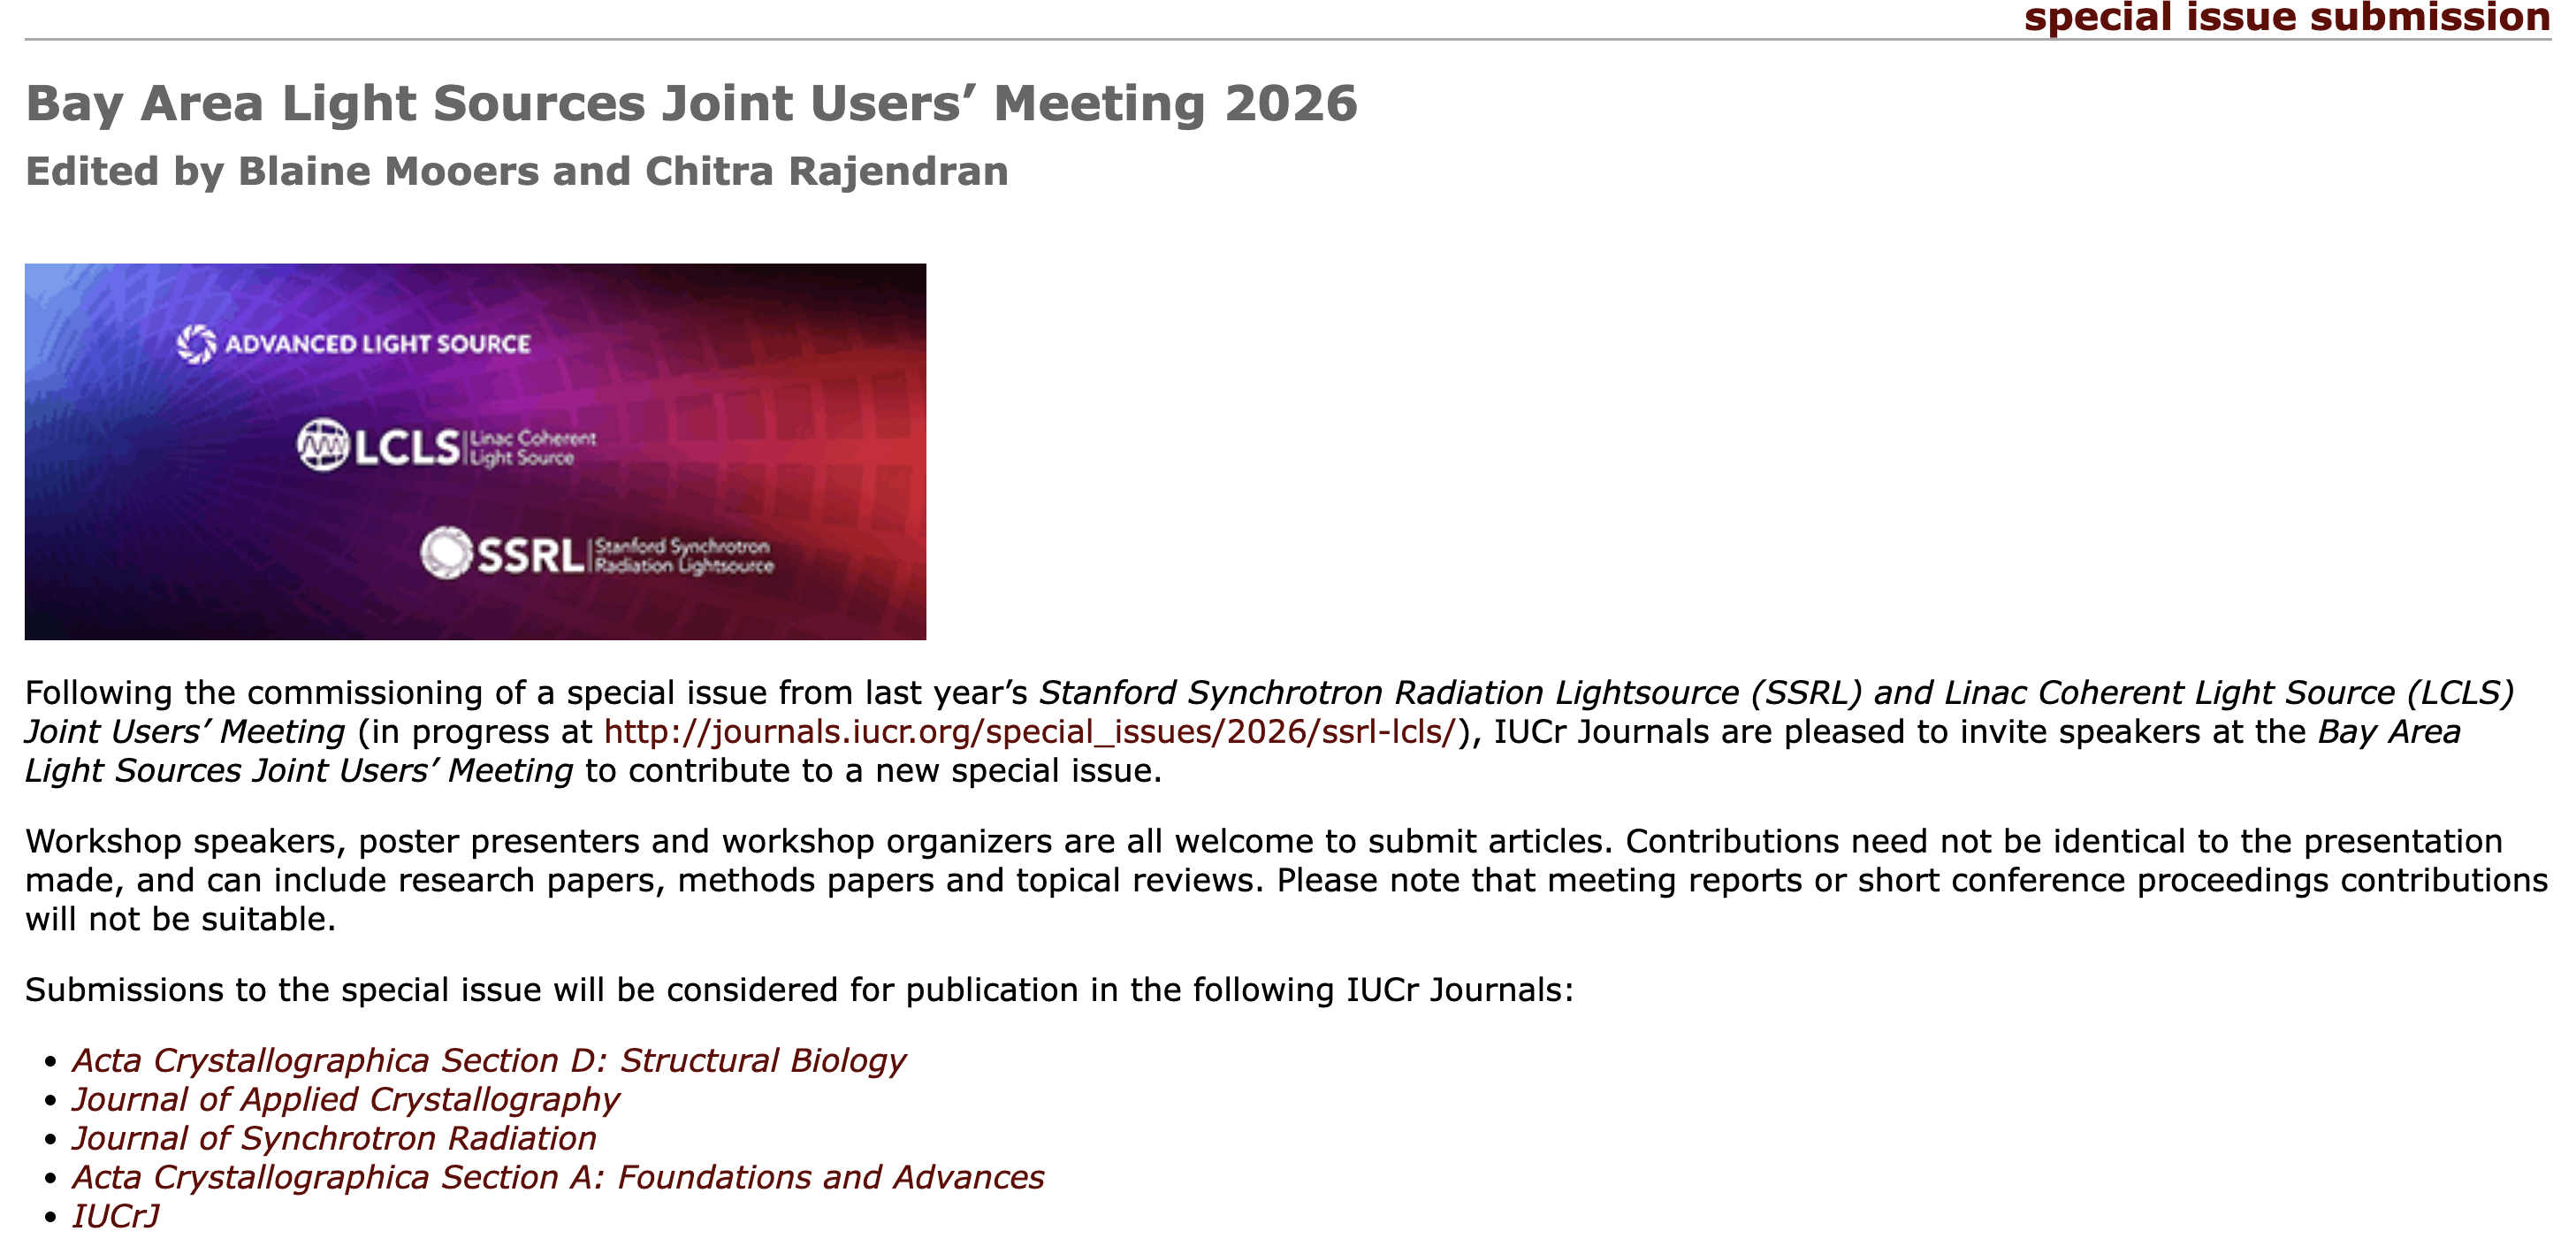
\includegraphics[width=0.95\linewidth]{./figs/VirutalIssue2026}
        % \caption{Ambient occlusion shortcuts AO and AOD.}
      \end{figure}
\footnotesize{\url{https://journals.iucr.org/special\_issues/submit/2027/ssrl-lcls/}}
\end{frame}

\end{document}

%%% Local Variables:
%%% mode: LaTeX
%%% TeX-master: t
%%% TeX-engine: xetex
%%% End:
